\section{Accuracy issues}

There are various accuracy issues when doing image rectification: 
\begin{enumerate}
    \item Noise and numerical errors: noise and numerical errors in the input data can affect the accuracy of the rectification process. 
        It's essential to preprocess and filter the data to minimize these issues.
    \item Little information: when choosing lines to identify vanishing points, it's crucial to select lines that are sufficiently far apart. 
        Choosing lines that are too close to each other can lead to inaccuracies in vanishing point estimation and rectification.
    \item Vanishing point near infinity: in cases where the vanishing point is nearly at infinity, it can be challenging to perform accurate affine rectification. 
        To address this issue:
        \begin{itemize}
            \item Draw two lines in the scene that are perpendicular to the given lines in the image.
                If the two new lines are not parallel, adjust one of the intersection points to make them parallel.
                \begin{figure}[H]
                    \centering
                    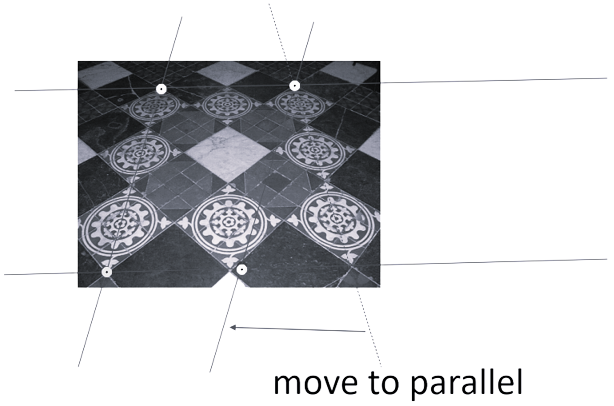
\includegraphics[width=0.4\linewidth]{images/vpi.png}
                \end{figure}
                Finally, apply affine reconstruction to obtain accurate results. 
                \begin{figure}[H]
                    \centering
                    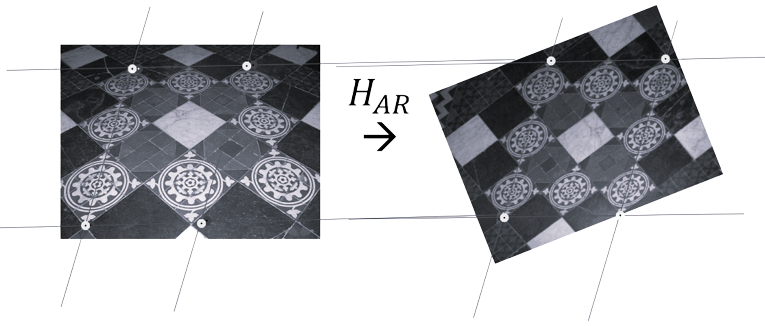
\includegraphics[width=0.5\linewidth]{images/ar.png}
                \end{figure}
            \item When dealing with sets of parallel lines, you can choose one line from each set and randomly select another pair of lines, making sure they are perpendicular. 
                With these four lines, you can compute the matrix product of $K$ and its transpose, denoted as $KK^T$, and then derive $K$ through Cholesky factorization.
                Afterward, you can apply the rectifying transformation using the matrix:
                \[H_{rect}=\begin{bmatrix}
                    K & t \\ 
                    0 & 1
                \end{bmatrix}^{-1}\] 
        \end{itemize}
\end{enumerate}
The accuracy of image rectification is crucial for various computer vision and image processing applications, and addressing these issues is essential for obtaining reliable results.